\documentclass{beamer}
\usepackage[landscape, margin=2cm]{geometry}
\usepackage{color}
\usepackage{bm}
\usepackage{graphicx}
\usepackage{hyperref}
\usepackage{listings}
\definecolor{mygreen}{rgb}{0,0.6,0}
\definecolor{mymauve}{rgb}{0.58,0,0.82}
\lstset{ %
  backgroundcolor=\color{white},   % choose the background color; you must add \usepackage{color} or \usepackage{xcolor}
  basicstyle=\footnotesize,        % the size of the fonts that are used for the code
  commentstyle=\color{mygreen},    % comment style
  deletekeywords={...},            % if you want to delete keywords from the given language
  extendedchars=true,              % lets you use non-ASCII characters; for 8-bits encodings only, does not work with UTF-8
  frame=single,                    % adds a frame around the code
  keywordstyle=\color{blue},       % keyword style
  language=Python,                 % the language of the code
  rulecolor=\color{black},         % if not set, the frame-color may be changed on line-breaks within not-black text (e.g. comments (green here))
  showspaces=false,                % show spaces everywhere adding particular underscores; it overrides 'showstringspaces'
  stringstyle=\color{mymauve},     % string literal style
  title=\lstname                   % show the filename of files included with \lstinputlisting; also try caption instead of title
}
\hypersetup{
    colorlinks=true,
    urlcolor=blue
}

\graphicspath{ {./img/} {./charts/} }


\title{How Complex Systems Fail}
\author{Adam Johnson - me@adamj.eu}
\date{18th March 2015}

\begin{document}

\maketitle


% Introduction

\frame{
    \frametitle{Introduction}
    \framesubtitle{Me}

    \begin{itemize}
        \item Developer/DBA/Ops at YPlan
    \end{itemize}
}

\frame{
    \frametitle{Introduction}
    \framesubtitle{Tonight's Paper}

    \begin{itemize}
        \item ``How Complex Systems Fail'' by Richard I. Cook
    \end{itemize}
}

\frame{
    \frametitle{Introduction}
    \framesubtitle{Tonight's Paper}

    \begin{center}
        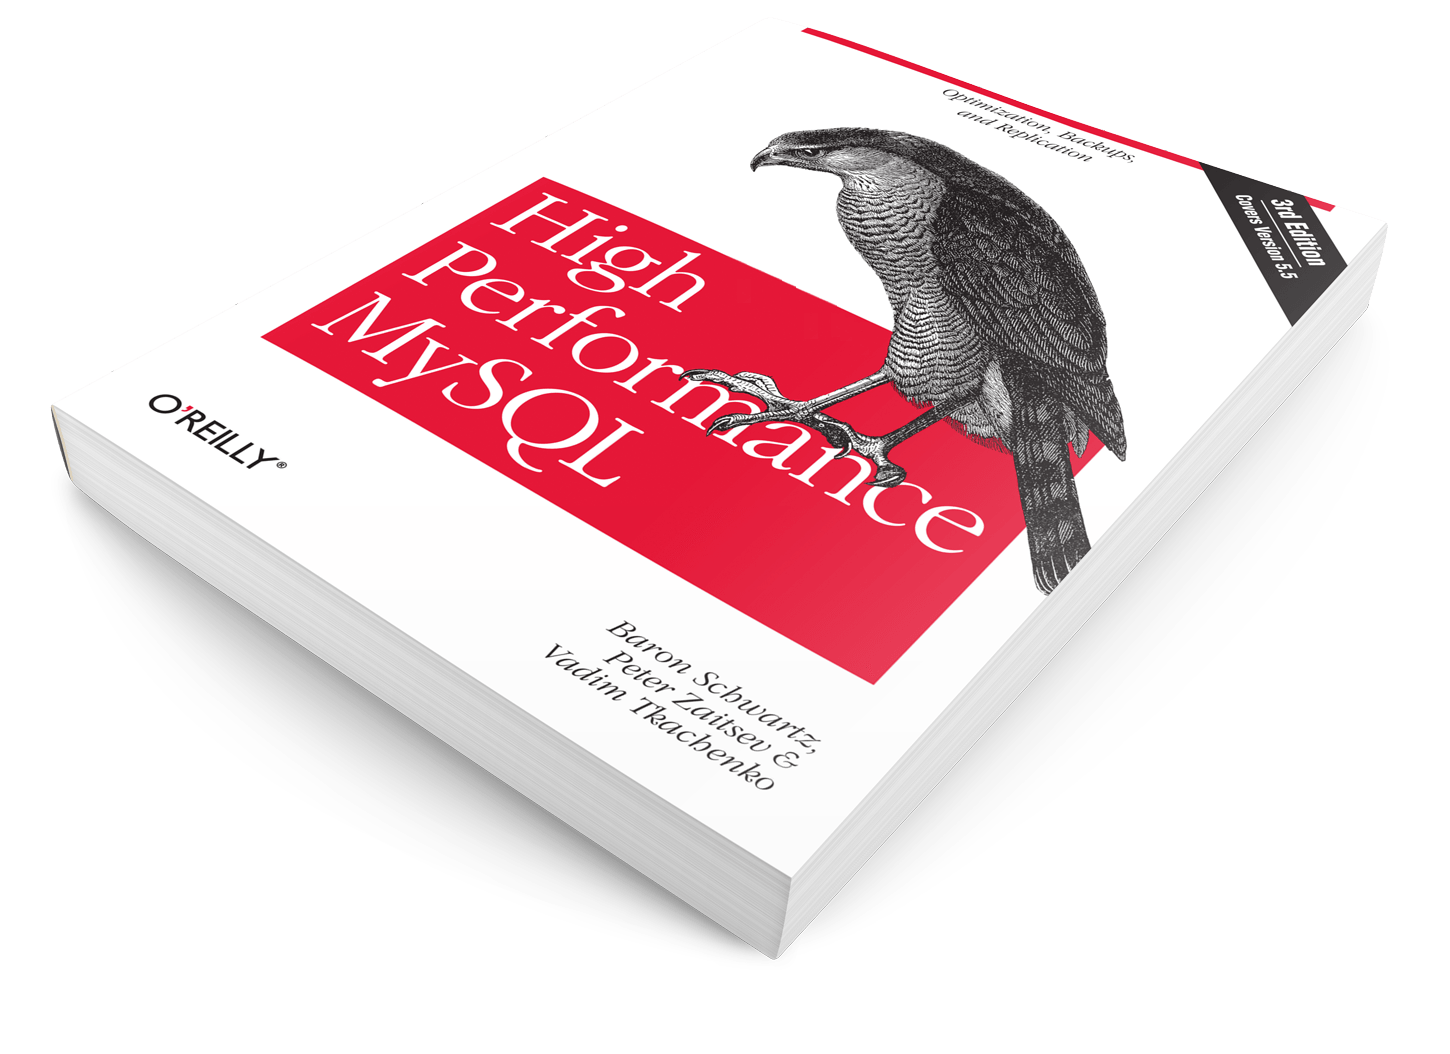
\includegraphics[width=9cm]{hpm-cover-perspective}
    \end{center}
}

\frame{
    \frametitle{Introduction}
    \framesubtitle{This Talk}

    \begin{enumerate}
        \item The Paper
        \item Computer Systems
        \item Nuclear Weapons
    \end{enumerate}
}

\frame{
    \frametitle{Introduction}
    \framesubtitle{Launch Complex 374-7, Little Rock Air Base, Arkansas}

    \begin{center}
        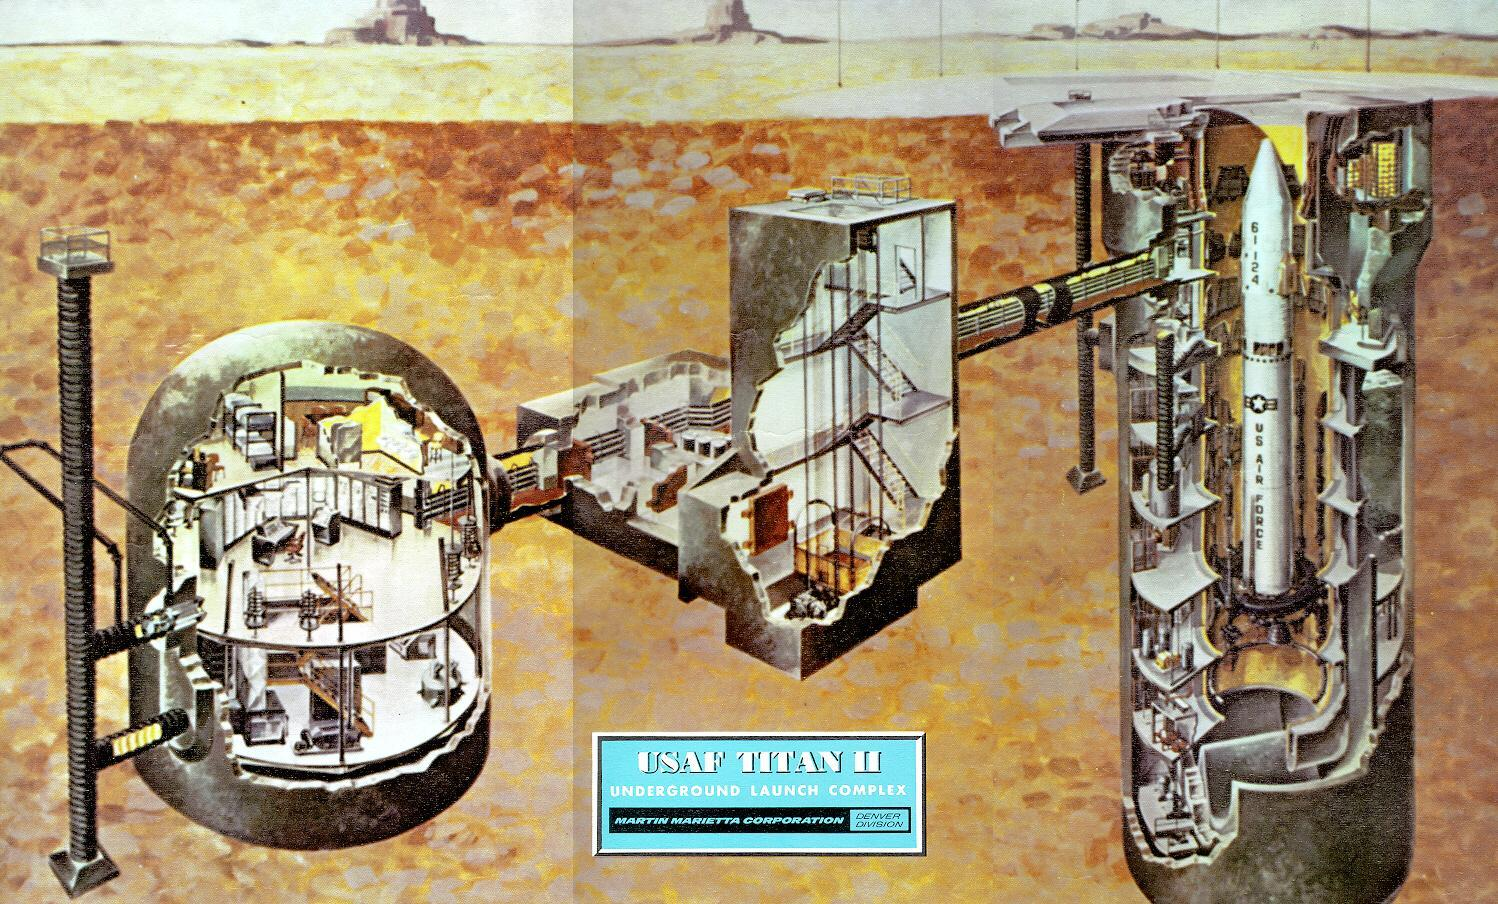
\includegraphics[width=10cm]{titan2bunker}
    \end{center}
}


% Conclusion

\frame{
    \frametitle{Thank you}

    \begin{itemize}
        \item \url{me@adamj.eu}
    \end{itemize}
}


\end{document}
